\documentclass[14pt]{beamer}

% Presento style file
\usepackage{config/presento}
% custom command and packages
\input{config/custom-command}
% My macros
/Users/zach/Git/zachs_macros/zachs_macros.tex

% Custom colors
\usepackage{color}
\definecolor{ao}{rgb}{0.0, 0.5, 0.0}

% Configure listings for R
\usepackage{listings}

\lstset{frame=tb,
language=R,
keywordstyle=\color{blue},
otherkeywords={!,!=,~,$,*,\&,\%/\%,\%*\%,\%\%,<-,<<-,\%>\%},
alsoletter={.,_}
}

% For hierarchical lists
\usepackage{outlines}

% Information
\title{LOST IN HYPERSPACE}
\subtitle{\emph{The Curse of Dimensionality}}
\author{Zachary del Rosario}
\institute{zdr@stanford.edu}
\date{September 6th}
%% \date{\today}

% For latex 2018
\makeatletter
\let\@@magyar@captionfix\relax
\makeatother

% --------------------------------------------------
\begin{document}
% --------------------------------------------------
\begin{frame}[plain]
\maketitle
\end{frame}

% --------------------------------------------------
%% SEC: Introduction
% --------------------------------------------------
\begin{frame}[t]{Thought Experiment: Parameter Study}
  Input variables $\vx\in\R{d}$ \\
  Scalar simulation output $f(\vx)$ \\
  Full factorial: $d$ input variables, $10$ points per dimension \\

  \bigskip
  \only<2>{%
    \centering
    \includegraphics[width=0.4\textwidth]{../images/points1}
  }
  \only<3>{%
    \centering
    \includegraphics[width=0.4\textwidth]{../images/points2}
  }
  \only<4>{%
    Scaling is \emph{exponential}, i.e.
    \begin{equation*}
      \text{Time} = (10\text{ seconds})^d
    \end{equation*}
  }
\end{frame}

% -------------------------
\begin{frame}{Computational Time}
  \visible<2>{The Curse of Dimensionality}
  \begin{table}
    \begin{tabular}{r|r|l}
    \hline
    Dimension & Time (s) & Comparison\\
    \hline
    1 & 1.0e+01 & Ten seconds\\
    \hline
    5 & 8.6e+04 & One Day\\
    \hline
    10 & 1.0e+10 & Eleven generations\\
    \hline
    18 & 4.3e+17 & Age of Universe\\
    \hline
    20 & 1.0e+20 & 230 x AoU\\
    \hline
    \end{tabular}
  \end{table}
\end{frame}

% -------------------------
\begin{frame}{UQ Tasks}
  High-dimensional integrals
  \begin{itemize}
  \item Moments $\E[\mX^n]$
  \item Probabilities $\E[\i1(\mX<x)]$
  \end{itemize}

  \bigskip Quadrature via full factorial (tensor grid) is exponential \\
  We need to address the Curse
\end{frame}

% -------------------------
\begin{frame}{Speaker Goals}
  \begin{itemize}
  \item Motivate
  \item Details and pointers
  \item New stuff
  \end{itemize}
\end{frame}

% -------------------------
\begin{frame}{Outline}
  \begin{outline}
  \1 UQ Tasks (Done)
  \1 Curse of Dimensionality
    \2 High-dimensional geometry
  \1 Lifting the Curse
    \2 Dimension reduction
  \end{outline}
\end{frame}

% --------------------------------------------------
%% SEC: Curse of Dimensionality
% --------------------------------------------------
\begin{frame}{Background}
  \begin{outline}
  \1 ``Curse of Dimensionality'' -- Richard Bellman (1961) \\
  \1 \emph{Vague} term
    \2 Integration
    \2 Sampling
    \2 Machine Learning
    \2 Distance
    \2 Big data
  \end{outline}
\end{frame}

% -------------------------
\framecard[colorblue]{{\color{white}%

``The trend today is towards more observations \emph{but even more so},
    \alert{to radically larger numbers of variables} – voracious, automatic,
    systematic collection of hyper-informative detail about each observed
    instance.''

    \bigskip
    -- David Donoho, 2000\\
    \tiny (Emphasis added)

}}

% -------------------------
\begin{frame}{My Point}
  Curse of Dimensionality is \emph{everywhere} \\
  Lots of \emph{very different} perspectives

  \bigskip
  So what's up with high dimensions?
\end{frame}

% -------------------------
\framecard[colorgreen]{{\color{white}\hugetext{%
      \centering%
      Weird Facts\\
      about\\
      High-\\
      Dimensional\\
      Geometry
}}}

% -------------------------
\begin{frame}{Fact 1}
  The hypersphere has vanishing interior
\end{frame}

% -------------------------
\begin{frame}{Unit Hypersphere Volume}
  \begin{equation*} \begin{aligned}
      HV &= \int\cdots\int \alert{r^{d-1}}\,
           T(\varphi_{1},\dots,\varphi_{d-1})\,
           dr d\varphi_{1}\cdots d\varphi_{d-1}
  \end{aligned} \end{equation*}
\end{frame}

% -------------------------
\framepicv[0.8]{../images/surface_density}{}

% -------------------------
\begin{frame}{Fact 2}
  The hypersphere concentrates at \emph{the} equator
\end{frame}

% -------------------------
\framepicv[1.0]{../images/great_circle}{
 \begin{textblock}{7}(0.0,5.7)
    {\tiny By P.wormer}
 \end{textblock}
}

% -------------------------
\begin{frame}{A Wordgame}
  \emph{An} equator is always $d-1$ dimensional \\

  \bigskip An epsilon-band around a great circle can be made to hold an
  arbitrary volume-fraction
\end{frame}

% -------------------------
\framepicv[0.8]{../images/equator}{}

% -------------------------
\begin{frame}{Fact 3}
  Johnson-Lindenstrauss Lemma:

  \bigskip \emph{Random projections} preserve \\
  \emph{pairwise distances}
\end{frame}

% JL: Example
% -------------------------
\begin{frame}[fragile]{JL: Example}
Example: Gene expression levels for some tumor types

\bigskip
  \begin{lstlisting}
## Gene data from UCI
dim(gene_data)
#       Obs,  Dim
> [1]   801 20531
  \end{lstlisting}

  \bigskip
  Note: This code on GitHub: https://github.com/zdelrosario/hyperspace
\end{frame}

% -------------------------
\begin{frame}[fragile]{JL: Example}
  \begin{lstlisting}
eps <- 0.1             # 10% distort
n <- dim(gene_data)[1] # Observations
d <- dim(gene_data)[2] # Dimension

k <-  2 * ceiling(C * log(n) / eps ^ 2)
k
# Intrinsic dimensionality
> 1338 (6.5% of 20531)
  \end{lstlisting}
\end{frame}

% -------------------------
\begin{frame}[fragile]{JL: Example}
  \begin{lstlisting}
## Randomly project
P_k <- random_projection(k x d)
## Project
projected_data = gene_data %*% P_k
## Match mean distances
a <- mean_distance(gene_data) /
  mean_distance(projected_data)
projected_data = a * projected_data
  \end{lstlisting}
\end{frame}

% -------------------------
\begin{frame}[fragile]{JL: Example}
  \begin{lstlisting}
eps
# Requested distortion
>    10%
quantile(relative_difference)
# Quantile
>      0%     25%    50%    75%   100%
# Realized distortion
> -7.784% -1.193% 0.082% 1.344% 8.139%
  \end{lstlisting}
\end{frame}

% -------------------------
\begin{frame}{Why Does This Work?}
  \underline{Claim}: For any $0<\epsilon<1$ and $n\in\mathbb{Z}_{>0}$, let
  $k\in\mathbb{Z}_{>0}$ such that

  \begin{equation*}
    k \geq C \frac{\log(n)}{\epsilon^2},
  \end{equation*}

  \noindent then for all sets of points $V\subset\R{d}$, there is a projection
  $P_k:\R{d}\to\R{k}$ such that, for all $u,v\in V$, we have

    \begin{equation*}
      \alert<2>{(1 - \epsilon)\|\vu - \vv\|^2 \leq \alpha\|P_k(\vu) - P_k(\vv)\|^2 \leq %
      (1 + \epsilon)\|\vu - \vv\|^2
}    \end{equation*}
\end{frame}

% JL: Distance
% -------------------------
\begin{frame}{}
  % Content
  \only<-5>{%
    \begin{equation*} \begin{aligned}
        (1 - \alert<3>{\epsilon})(\alert<2>{\text{Distance}})^2 &\leq %
          \alpha(\alert<4,5>{\text{Projected Distance}})^2 \\
        &\, \\
        \alpha(\alert<4,5>{\text{Projected Distance}})^2 &\leq %
          (1 + \alert<3>{\epsilon})(\alert<2>{\text{Distance}})^2\\
    \end{aligned} \end{equation*}
  }%
  % Annotation
  \visible<2-5>{%
    \begin{textblock}{3}(+1.5,-5.7)
      {\textblockcolor{}
        \centering%
        \only<2>{\includegraphics[width=1.0\textwidth]{../images/proj0_alert}}
        \only<3-5>{\includegraphics[width=1.0\textwidth]{../images/proj0}}
      }
    \end{textblock}
  }
  \visible<3-5>{%
    \begin{textblock}{3}(+5.5,-4.0)
      {\textblockcolor{}
        \alert<3>{$\epsilon$ is \emph{small}}
      }
    \end{textblock}
  }
  \visible<4-5>{%
    \begin{textblock}{3}(-0.5,+0.0)
      {\textblockcolor{}
        \centering%
        \only<4>{\includegraphics[width=1.0\textwidth]{../images/proj1_alert}}
        \only<5>{\includegraphics[width=1.0\textwidth]{../images/proj1}}
      }
    \end{textblock}
  }
  \visible<5-5>{%
    \begin{textblock}{3}(+3.0,+0.0)
      {\textblockcolor{}
        \centering\includegraphics[width=1.0\textwidth]{../images/proj2_alert}
      }
    \end{textblock}
  }
\end{frame}

% JL: Projections
% -------------------------
\begin{frame}[t]{}
  % Content
  \begin{equation*}
    (1 - \epsilon)\|\vu - \vv\|^2 \leq %
    \alert{\alpha}\|P_{\alert{k}}(\vu) - P_{\alert{k}}(\vv)\|^2 \leq %
    (1 + \epsilon)\|\vu - \vv\|^2
  \end{equation*}
  % Annotation
  \visible<2->{%
    \begin{textblock}{6}(+2.5,-0.5)
      {\textblockcolor{}
        \centering%
        \only<2>{\includegraphics[width=1.0\textwidth]{../images/dim_proj3}}
        \only<3>{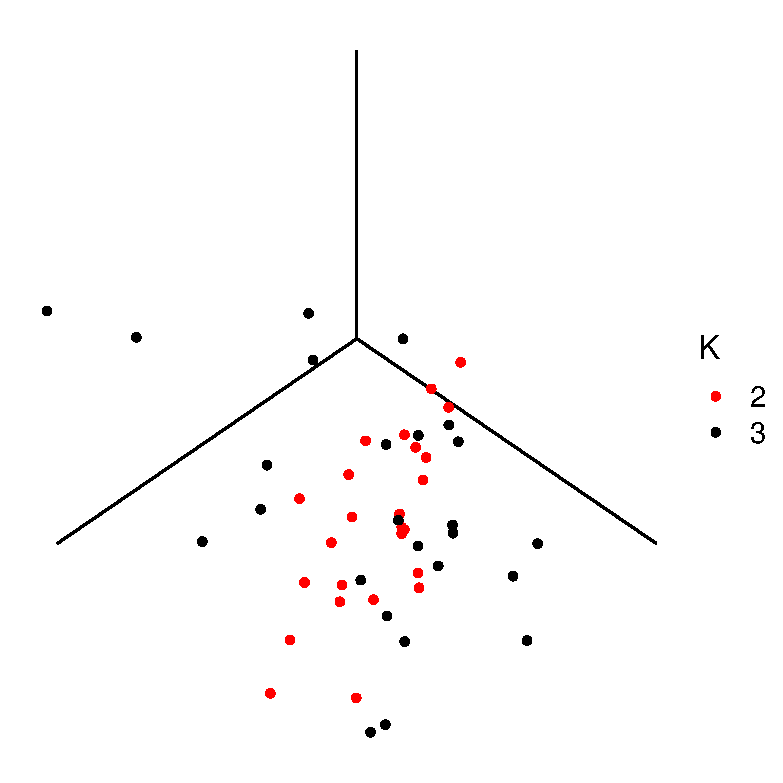
\includegraphics[width=1.0\textwidth]{../images/dim_proj2}}
        \only<4>{\includegraphics[width=1.0\textwidth]{../images/dim_proj1}}
      }
    \end{textblock}
  }
\end{frame}

% JL: Dimensionality
% -------------------------
\begin{frame}{}
  % Content
  \begin{equation*}
    \alert<2>{k} \geq C\frac{\log(\alert<3>{n})}{\alert<4>{\epsilon}^2}
  \end{equation*}
  % Annotation
  \visible<2->{%
    \begin{textblock}{4}(+0.0,-3.5)
      {\textblockcolor{}
        $k$ is the projection dimension
      }
    \end{textblock}
  }
  \visible<3->{%
    \begin{textblock}{4}(+0.0,+2.0)
      {\textblockcolor{}
        $n$ is the number of observations
      }
    \end{textblock}
  }
  \visible<4->{%
    \begin{textblock}{4}(+7.0,+2.0)
      {\textblockcolor{}
        $\epsilon$ is the desired error
      }
    \end{textblock}
  }
  \visible<5->{%
    \begin{textblock}{4.5}(+7.0,-3.5)
      {\textblockcolor{}
        Dimensionality is\\
        \emph{curiously absent!}
      }
    \end{textblock}
  }
  \visible<6>{%
    \begin{textblock}{4.5}(+3.5,-0.0)
      {\textblockcolor{}
        $k$ is an \emph{intrinsic dimensionality}
      }
    \end{textblock}
  }
\end{frame}

% --------------------------------------------------
%% SEC: Dimension Reduction
% --------------------------------------------------
\framecard[colorgreen]{{\color{white}\hugetext{%
      \centering%
      Lifting\\
      the\\
      Curse: \\

      \bigskip
      \alert{Dimension Reduction}
}}}

% -------------------------
\begin{frame}{Dimension Reduction}
  Idea: Identify low-dimensional structure; reduce effective dimension \\
  If $\text{Cost} = C^d$, then reduce $d$
\end{frame}

% -------------------------
\begin{frame}{Dimension Reduction \alert{In UQ}}
  \bigskip \textcolor{green}{J-L showed us \emph{linear} low-dimensional structure} \\
  \textcolor{red}{J-L does not separate \emph{inputs} and \emph{response}}

  \bigskip We've talked about $\vx$ \\
  What about $f(\vx)$?
\end{frame}

% -------------------------
\begin{frame}{DR Taxonomy}
  \begin{outline}
  \1 Generic-space DR (J-L, PCA, etc.)
    \2 No additional structure on $\R{d}$
  \1 Output-space DR (ROMs, POD, etc.)
    \2 $\R{d}$ is state space, often temporal structure
  \1 \alert<2>{Input-space DR} (...)
    \2 $\R{d}$ is input space, connected to response
  \end{outline}
\end{frame}

% -------------------------
\begin{frame}{Running Example: Pipe Flow}
  \centering
  \includegraphics[width=0.9\textwidth]{../images/pipe_diagram}

  \visible<2>{%
    \begin{textblock}{4.5}(+0.5,+0.5)
      {\textblockcolor{}
        qoi: (normalized) pressure loss
        inputs: $\rho, u, d, \mu, \epsilon$
      }
    \end{textblock}
  }
\end{frame}

% -------------------------
\begin{frame}{Dimension Reduction: Methods}
  \begin{outline}
    \1 Subset reduction
      \2 Morris screening
      \2 Sobol' indices
    \1 Subspace reduction
      \2 PCA-primer
      \2 Active subspaces
  \end{outline}
\end{frame}

% -------------------------
\begin{frame}{Subset Reduction}
  Suppose $\vx^{\top} = [\vx_A^{\top}, \vx_I^{\top}]$ \\
  What if some variables were \emph{inactive}? E.g.

  \begin{equation}
    f(\vx_A, \vx_I) = f(\vx_A, \vx'_I),
  \end{equation}

  \noindent for all $\vx_I \neq \vx'_I$. Can then \emph{ignore} $\vx_I$.
\end{frame}

% -------------------------
\begin{frame}{Subset Reduction: Methods}
  \begin{outline}
    \1 Morris screening
      \2 \textcolor{green}{Inexpensive}
      \2 \textcolor{red}{Difficult to interpret}
    \1 Sobol' indices
      \2 \textcolor{green}{Clear interpretation}
      \2 \textcolor{red}{Can be expensive}
  \end{outline}
\end{frame}

% -------------------------
\begin{frame}{Sobol' Indices}
  Idea: Attribute \emph{variance in output} $f$ to \emph{different inputs}

  \bigskip E.g.
  \begin{table}
    \centering
    \begin{tabular}{@{}llllll@{}}
     & $\rho$ & $U$ & $d$ & $\mu$ & $\epsilon$\\
    \hline
    Var & 0\% & 0\% & 6\% & 0\% & 94\% \\
    \end{tabular}
  \end{table}

  How to \emph{attribute} variance?
\end{frame}

% -------------------------
\begin{frame}{Sobol' Formulation}
  Variance decomposition
  \begin{equation}
    \V[Y^2] = \E[\V[Y|\mX_{\vu}]] + \V[\E[Y|\mX_{\vu}]]
  \end{equation}

  First-order index
  \begin{equation}
    \underline{\tau}_{\{i\}}^2 = \frac{\V[\E[Y|X_i]]}{\V[Y]}.
  \end{equation}

  Total-order index
  \begin{equation}
    \overline{\tau}_{\{i\}}^2 = \frac{\E[\V[Y|X_{-\{i\}}]]}{\V[Y]}
  \end{equation}
\end{frame}

% -------------------------
\begin{frame}{But wait...}
  Sobol' indices based on \emph{variance}... \\
  Variance is an \emph{expectation}... \\

  \bigskip Sobol' is cursed by dimensionality!
\end{frame}

% -------------------------
\begin{frame}{Subspace Reduction: Methods}
  \begin{outline}
    \1 Principal Component Analysis (PCA)
      \2 Intuition
    \1 Active subspaces
      \2 Application
  \end{outline}
\end{frame}

\end{document}
